%
% File: chap01.tex
% Author: Victor F. Brena-Medina
% Description: Introduction chapter where the biology goes.
%
\let\textcircled=\pgftextcircled
\chapter{Introduction}
\label{chap:intro}

\initial{T}he technique of automatic video content analysis (VCA) is one of the most important areas of Computer Vision and Artificial Intelligence. With this technique, machines can recognize objects, human activities and events in videos.   Thus, it can be widely used in many domains, such as human-computer interaction, video classification, entertainment, self-driving, public safety and security, home automation, etc. Action and interaction analysis is one of the most common uses of VCA which focus on human activities analysis, including action recognition/detection of a single person or interaction recognition/detection of two or more people.


%=======
\section{Background}
\label{sec:intro_sec01}
When we talk about human action, we usually mean the activity of a single person. While human interaction is more complex which generally contains three cases: human-human interaction among two or more people like hand-shaking between two people, human-object-human interaction like one person pass an object to another one, and human-object interaction like one person push a table. 
\par 
The goal of \textbf{human action/interaction recognition} in a video is to determine the action/interaction label for a video that is what are the people doing in the video. And the goal of \textbf{human action/interaction detection} in a video is to localize a specific action/interaction spatially and temporally in a video. 
\par 
Although a lot of excellent methods and datasets were published in the last decade in the area of action recognition, it is still challenging and far from being solved. Comparatively, the related work in the domain of interaction recognition and detection is relatively scarce. This is because the job of interaction recognition and detection is even more challenging than that of action.  
 
\par
The main challenges of action and interaction recognition and detections in real scenes mainly include: 
\begin{enumerate}
	\item Various camera views, the videos which will be analysed could be taken from different viewpoints which have never been seen in training data. For example, Figure \ref{fig:challenges} (a) illustrates four videos of a same biking little girl being filmed from four different camera views. The features extracted from these videos can be various, then it becomes hard for the classifier to learn to discriminate them as same activity. 
	\item Complex background, the background of the interested action and interaction could be various and even totally different. For example, Figure \ref{fig:challenges} (b) illustrates four diving videos taken from totally different background with large camera motion. For those feature descriptors which extract features from not only the segmented person but also the background. Then the features extracted from background would largely confuse the classification results.  
	\item Usually, a single action video clip contains hundreds and even more frames, therefore there might be many irrelevant frames which would confuse the analysis. For instance, a video clip of playing basketball may contain frames of commentators and audiences. 
	\item It is hard to get a decent performance on a small training set. But sometimes we only have small scale target dataset with very limited training set. Such situation is even worse for the task of interaction video analysis since the related dataset is scare compared with action video analysis.
	\item Compared with action video analysis, extra features like the relative position and orientation between people involved in the interaction need to be taken into consideration, which makes the feature representation more complex. 
\end{enumerate}

\begin{figure}
	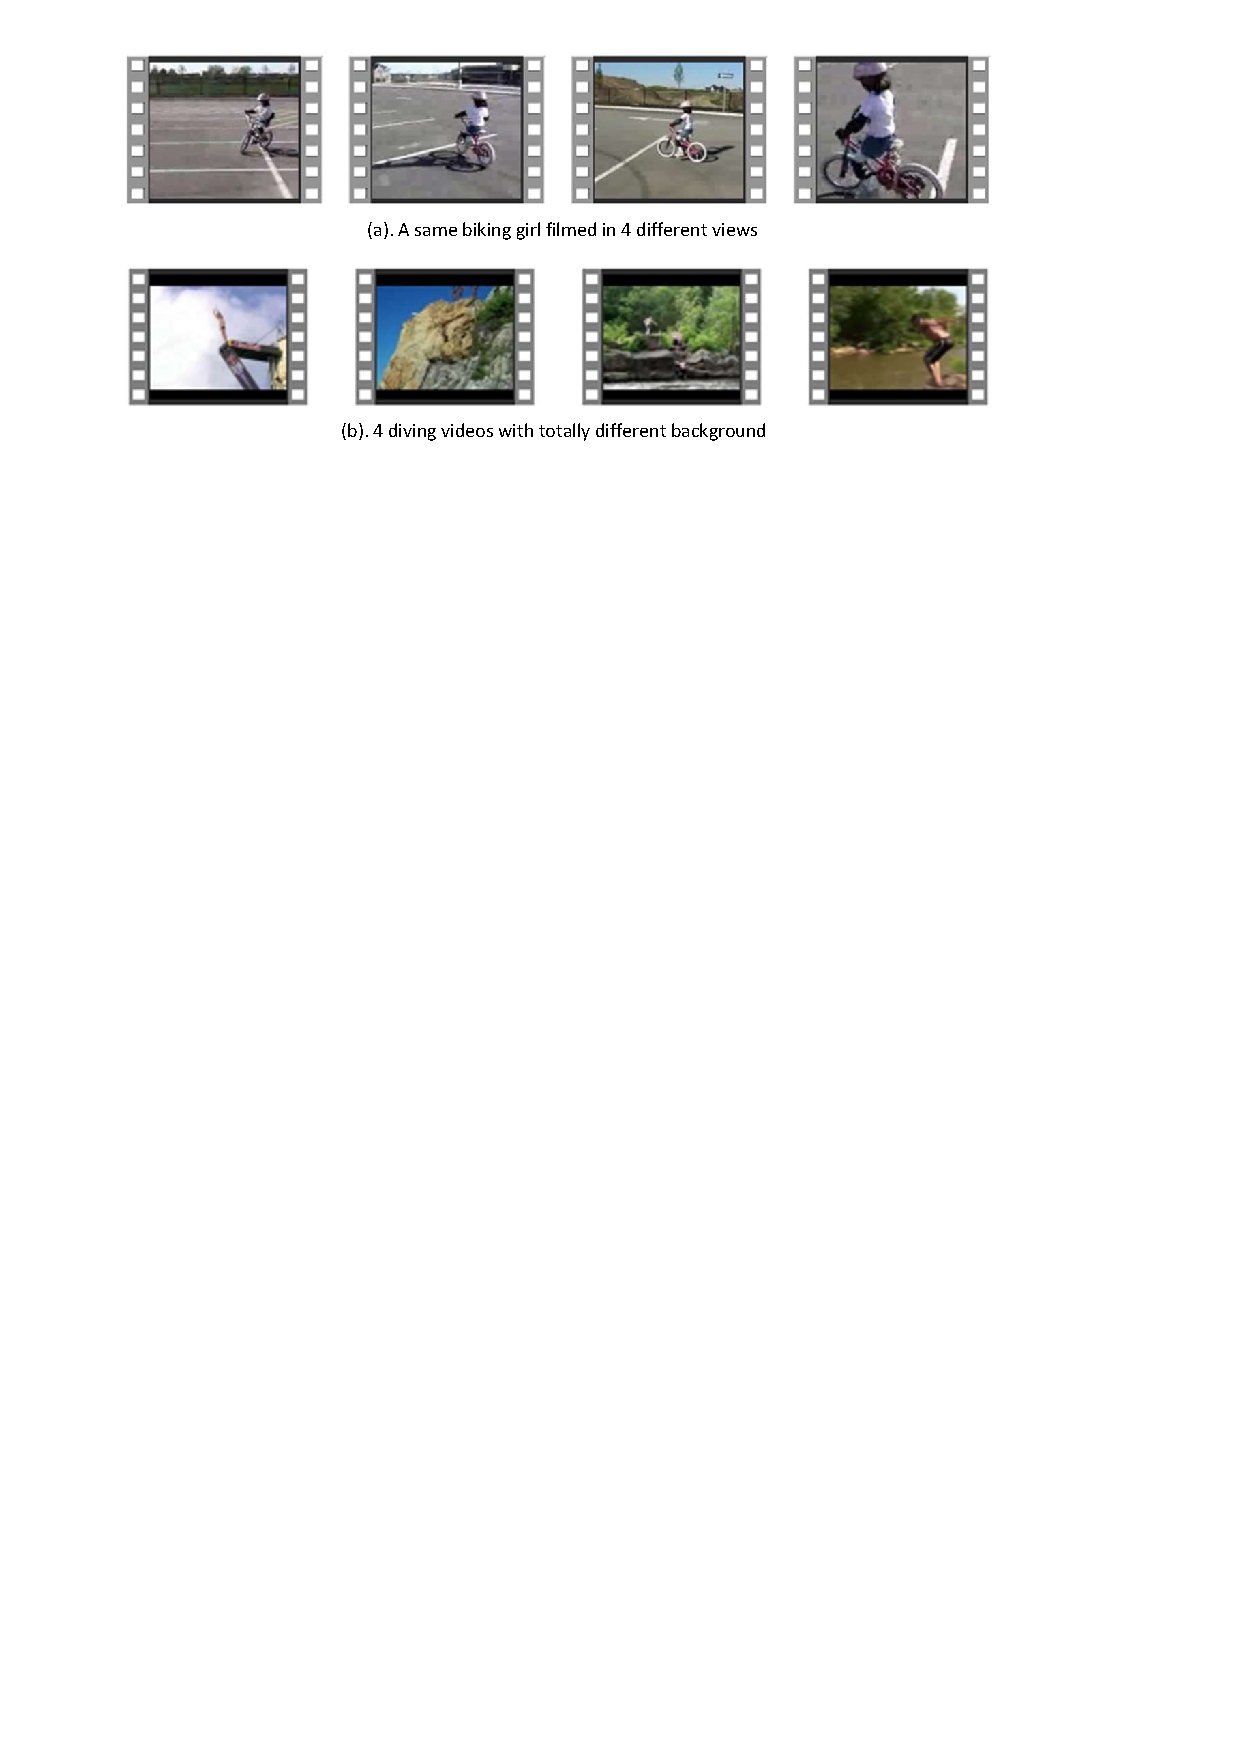
\includegraphics[trim=2cm 22cm 0cm 1cm]{fig01/challenges.pdf}
	\caption{Illustration of some challenges of video analysis. }
	\label{fig:challenges}
\end{figure}

Some of interaction analysis related works are \cite{patron2010}, \cite{Gemeren2015}, \cite{narayan2014} and \cite{choi2012}. Where the works of Patron-Perez et al. \cite{patron2010} and  Gemeren et al. \cite{Gemeren2015} focus on relative information between people involved in the interaction, such as relative position and orientation in relevant body parts, then use hand-crafted features descriptors, like histograms of orientated gradients (HOG \cite{hog}) and histograms of optical flow (HOF \cite{hof}), to describe those interaction features. The work of Narayan et al.  \cite{narayan2014} combines improved trajectory features and foreground motion map features to describe interaction features. Differently, Choi et al. \cite{choi2012} introduce a hierarchical method, which first detects and tracks the location of each person, then learns to analysis the atomic action for each person, and last use the atomic action to infer the collective interaction label. The atomic action is also represented by hand-crafted feature descriptors, such as HOG and bag of video words (BoV \cite{bov}).
\par 
In this thesis project, we adopt the similar hierarchical architecture with the work of Choi et al. with two main changes: 1). we use deep learning feature descriptors to represent the atomic action for each person involved in the interaction instead of hand-crafted feature descriptors; 2). Besides the networks learning atomic features for each person, we add  an additional deep learning network to learn the relative position and orientation features.   

\section{Project Goals}
\label{sec:intro_sec02}

In this thesis project, we will focus on two-person interaction recognition and detection. The goals of this thesis project including: 
\begin{enumerate}
	\item Do interaction recognition based on the target dataset. The inputs are the segmented specific interaction videos and the outputs are the predicted class labels.
	\item Do interaction detection based on the target dataset. The input is the un-segmented videos and the output is the spatial and temporal location of specified classes. 
	\item Construct a hierarchical multi-level network to learn interaction features. Hierarchical network means we first learn atomic action features for each person involved in interaction, then combine these features to learn interaction features. Multi-level network means we have global first level network which learns global interaction features, such as relative position and orientation between people involved in the interaction and second level network which learns atomic actions for each person.
\end{enumerate}

\section{Contributions}
\label{sec:intro_sec03}

We mainly have following contributions on interaction video analysis: 
\begin{enumerate}
	\item We introduce deep learning feature descriptors to address interaction recognition and detection with only small scale target interaction video dataset available. 
	\item We introduce a hierarchical multi-level framework for interaction video analysis tasks.
\end{enumerate}

\section{Outline}
\label{sec:intro_outline}
In the next chapter, we will introduce the action and interaction video analysis related works including methods and datasets. In Chapter \ref{chap3}, we will introduce our overall architecture, training strategies and the metric method of this project. In Chapter 4, we will descriptor the low-level design of this project in detail. In Chapter 5, we will introduce the training process and experiment results, and analyse the results. At last, we will give conclusions and possible future works of this project.
%=========================================================